\section{System Overview}
\label{sec:system}
\textsc{Synopsis} is implemented on top of Neptune stream processing system~\cite{buddhika2016neptune} as a specialized layer for geo-spatial data.
In this section, we will briefly introduce Neptune followed by a discussion on the design of \textsc{Synopsis}.

\subsection{Neptune}
Neptune is a distributed stream processing system which is optimized to process high throughput data streams.
It is designed to cope with application requirements such as high volumes of small stream packets, high and variable data rates and heterogeneity within stream processing jobs.
Satisfying these requirements imposes various system level challenges including possible buffer-overflow errors, increased number of context-switches, object creation overhead and memory management issues.
Neptune takes a holistic approach that considers CPU, memory, network and kernel issues to address the above challenges.
This is achieved through employing a set of optimizations such as application level buffering, batched scheduling, object re-use, built-in support for backpressure and selective compression to ensure a better utilization of system resources.

Users can deploy stream processing jobs as directed acyclic graphs in Neptune.
A stream processing graph consists of a set of stream ingestion points and stream processors (vertice) and streams connecting these operators (edges).
To provide each job with a initial load-balanced deployment plan to start with, each operator in a stream processing graph can be annotated with a parallelism level while each stream can be associated with a partitioning scheme.

\subsection{\textsc{Synopsis}}
\textsc{Synopsis} is a stream processing graph deployed on top of Neptune.
It is comprised of several stream ingestion operators and a dynamic set of stateful stream processors.
These stream processors collectively maintain the distributed sketch while the number of processors are dynamically adjusted by the \textsc{Synopsis} runtime to suit the changing operating conditions.
We use a stream partitioning scheme based on Geohash of stream packets to route stream packets to the appropriate stream processor which holds the corresponding section of the distributed sketch.

\textsc{Synopsis} extends the Neptune's generic stream processor to provide a set of auxiliary services required by its runtime.
These services are control plane, gossip subsystem and querying subsystem as depicted in Figure~\ref{fig:rivulet-archi}.
%
\begin{figure}
    \centerline{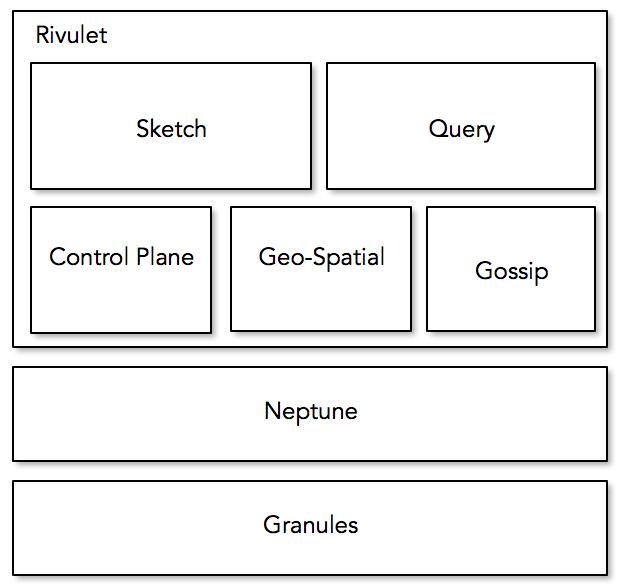
\includegraphics[scale=0.5]{figures/rivulet-archi.png}}
    \caption{\textsc{Synopsis} is implemented as a specialized layer for geo-spatial data on top of Neptune stream processing system.}
    \label{fig:rivulet-archi}
\end{figure}
%
\begin{description}[leftmargin=*]
	\item[Control plane:] Control plane is responsible for orchestrating control messages exchanged between \textsc{Synopsis} nodes as part of various distributed protocols such dynamic scaling.
	Control plane is decoupled from the data plane to ensure high priority and low latent processing without being affected by buffering delays and backpressure.

	\item[Gossip subsystem:] Majority of the \textsc{Synopsis} functionality is assumed to work with the local knowledge of a particular node, certain functionalities require an approximate global knowledge. 
	For instance, each \textsc{Synopsis} node maintains a prefix tree, to help the querying subsystem to know which nodes are holding the sections of the sketch responsible for the geohash locations corresponding to a query it evaluates (This is further explained in section~\ref{subsec:query-eval}). 
	In order to establish and maintain this global view of the entire system, \textsc{Synopsis} nodes gossip about their state periodically as well as when there is a change in the state which other nodes in the system are interested in.
	Given that there is a propagation and convergence delay inherent with the gossip protocols, at any given time, a \textsc{Synopsis} node will only have an eventually consistent view of the entire system.

	\item[Querying subsystem:] Querying subsystem is responsible for...
\end{description} 

Each Neptune process in the system host one or more \textsc{Synopsis} nodes.
A \textsc{Synopsis} node is essentially a task triggered to on the availability of data in any of its incoming streams.
Each \textsc{Synopsis} node is responsible for one of more sections of the distributed sketch as illustrated in Figure~\ref{fig:process-monitor}.
All \textsc{Synopsis} nodes running in a particular Neptune process is constantly probed by a monitoring task to gather their performance metrics: backlog information and memory utilization by individual sketches.
This information is used for dynamic scaling recommendations as explained in section~\ref{subsec:scaling-out}.

\begin{figure}
    \centerline{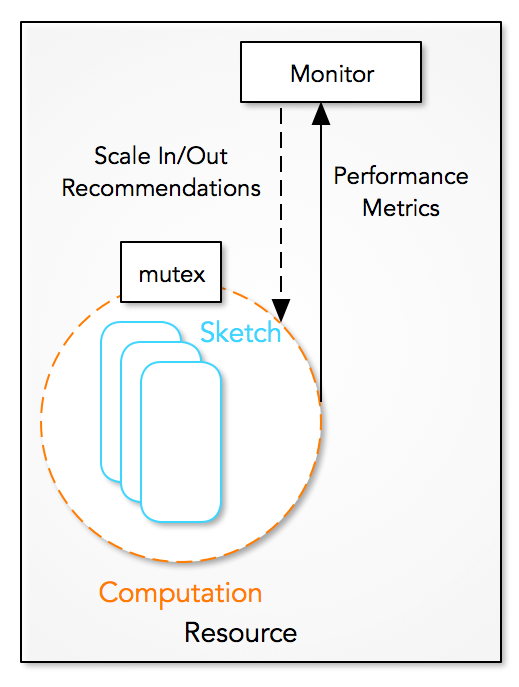
\includegraphics[scale=0.55]{figures/process-monitor.png}}
    \caption{Dynamic scaling is triggered by monitoring the backlog of each computation and memory pressure incurred in each process.}
    \label{fig:process-monitor}
\end{figure}